% ============================================================
% QM-6: Capstone — Four Primitives to Full QM
% Version 1.1 — 2 April 2026
%
% CHANGELOG:
%   v1   Mar 2026  — Initial draft
%   v1.1 2 Apr 2026 — Formatting compliance: .bib, natbib,
%                     graphicspath, TOC, PLS, OSF DOI
%
% FIGURE PATH:
%   .tex: series_quantum_mechanics/papers/
%   figs: series_quantum_mechanics/figures/figures-QM-6/
% ============================================================

\documentclass[11pt,letterpaper]{article}
\usepackage[margin=1in]{geometry}
\usepackage[utf8]{inputenc}
\usepackage[T1]{fontenc}
\usepackage{amsmath,amssymb,amsthm}
\usepackage{graphicx}
\usepackage{svg}
\svgsetup{inkscapelatex=false,inkscapeformat=pdf,inkscapepath=svgdir}

% Figure path: papers/ → ../figures/figures-QM-6/
\graphicspath{{../figures/figures-QM-6/}}

\usepackage{caption}
\usepackage{float}
\usepackage{booktabs}
\usepackage{longtable}
\usepackage{enumitem}
\usepackage{parskip}
\usepackage{xcolor}
\usepackage[authoryear,round]{natbib}
\usepackage{hyperref}
\hypersetup{colorlinks=true,linkcolor=blue,urlcolor=cyan,citecolor=red}

\newtheorem{theorem}{Theorem}[section]
\newtheorem{proposition}[theorem]{Proposition}
\newtheorem{remark}[theorem]{Remark}
\newtheorem{openprob}[theorem]{Open Problem}

\newcommand{\lP}{l_P}
\newcommand{\tP}{t_P}
\newcommand{\EP}{E_P}
\newcommand{\SSV}{\mathrm{SSV}}
\newcommand{\ket}[1]{|#1\rangle}

\title{\textbf{Quantum Mechanics in Conscious Point Physics:\\
Full Synthesis --- From Four Primitives to Quantum Field Theory}\\[6pt]
{\large QM Series --- Capstone (Version 3.1)}}

\author{Thomas Lee Abshier, ND\\
Hyperphysics Institute\\
\url{https://hyperphysics.com}\\
\texttt{drthomas007@protonmail.com}}

\date{22 March 2026}

\begin{document}
\maketitle

\begin{abstract}
All of quantum mechanics emerges in Conscious Point Physics from four
primitives: Conscious Points (CPs), phase-carrying Displacement
Increment (DI) bits, the 600-cell lattice, and the Nexus.  The
complex DI-bit amplitude $\psi_i = \sqrt{\rho_i}\,e^{i\phi_i}$
evolves by deterministic hopping, yielding the Schr\"{o}dinger
equation in the continuum limit (Paper~2~\cite{cpp2040a}).
Simultaneous propagation along all geodesics gives the discrete
Feynman path integral and quantum superposition
(Paper~3~\cite{cpp2040b_super}).  The Nexus maintains non-separable
joint DI-bit states, giving quantum entanglement and Bell violation
$|\mathrm{CHSH}|=2\sqrt{2}$ with no-signaling
(Paper~4~\cite{cpp2040c}).  DP~Sea decoherence produces apparent
collapse with pointer basis fixed at SSV eigenstates
(Paper~5~\cite{cpp2040d}).  Collective 600-cell eigenmodes give field
operators, commutation relations, and finite renormalization
(Paper~6~\cite{cpp2040e}).  All lattice corrections are
$\mathcal{O}((\lP/\lambda)^2)$ and unobservable at laboratory scales.
The hierarchy problem is finite; SM masses remain an open problem.
The entire QM sector is derived from four primitives with no new
postulates.
\end{abstract}

\medskip\noindent
\textbf{Keywords:} quantum mechanics foundations, four primitives, emergence of QM, Nexus constraint, Conscious Point Physics, derived vs postulated, lattice quantum mechanics

\bigskip\noindent
\textbf{Plain Language Summary:}
This paper summarises what CPP has achieved for quantum mechanics. Starting from just four ingredients — conscious points, the 600-cell lattice, DI-bit amplitudes, and the Nexus global constraint — the entire framework of quantum mechanics follows: the Schrödinger equation, the Born rule for probabilities, quantum interference, Bell inequality violations, decoherence and measurement, and quantum field theory with three generations. No additional postulates are needed beyond the four primitives. The remaining open problem is deriving Planck's constant from these four ingredients.

\bigskip
\raggedright
\tableofcontents
\newpage


\tableofcontents
\newpage

%=====================================================================
\section{The Four Primitives}
%=====================================================================

\begin{enumerate}
\item \textbf{Conscious Points (CPs)}: Planck-scale entities carrying
  charge $\pm e$.  Each occupies one Grid Point and executes local
  deterministic rules.

\item \textbf{Displacement Increment (DI) bits}: Relational quanta
  exchanged between CPs, carrying both density $\rho$ and geometric
  phase $\phi$.  The complex amplitude $\psi = \sqrt{\rho}\,e^{i\phi}$
  encodes the full DI-bit state at each Grid Point.

\item \textbf{600-cell lattice}: 120 Grid Points, 720 edges,
  coordination $z=12$, adjacency matrix with exactly six distinct
  eigenvalues $\{12, 1+\varphi, \varphi-1, 1-\varphi, -\varphi,
  -(1+\varphi)\}$ where $\varphi = (1+\sqrt5)/2$.

\item \textbf{Nexus}: Atemporal global constraint enforcing DI-bit
  number conservation and total phase circulation at every Absolute
  Moment tick.  Not a signal; not a hidden variable.
\end{enumerate}

%=====================================================================
\section{The Emergence Chain}
%=====================================================================

\subsection{Paper~2 --- Schr\"{o}dinger equation from lattice
hopping~\cite{cpp2040a}}

DI bits hop with phase accumulation $\Delta\phi = m_{\rm CP}c\Delta s/\hbar$.
The discrete evolution:
\begin{equation}
\psi_i(t+\Delta t) = \psi_i(t)
- \frac{i\Delta t}{\hbar}\sum_j H_{ij}\psi_j,
\quad H_{ij} = -T\;\text{(neighbours)},\;
T = \frac{\hbar^2}{4m\Delta s^2}.
\end{equation}
Via the 600-cell graph Laplacian
$\sum_{j\sim i}(\psi_j-\psi_i) = 2\Delta s^2\nabla^2\psi$:
\begin{equation}
i\hbar\partial_t\psi = -\frac{\hbar^2}{2m}\nabla^2\psi + V_{\SSV}\psi.
\end{equation}
\textbf{Key correction:} $T = \hbar^2/(4m\Delta s^2)$ (not $\hbar^2/(2m\Delta s^2)$)
to absorb the factor~2 from the 12-neighbour graph Laplacian.

\subsection{Paper~3 --- Superposition from multi-path
summation~\cite{cpp2040b_super}}

Each DI bit propagates simultaneously along all geodesics:
\begin{equation}
\psi(d) = \sum_k A_0\,e^{i\phi_k}.
\end{equation}
Interference from relative phases.  SSV gradient $=$ which-path tag.
Quantum eraser $=$ SSV cancellation.  Born rule: $P = |\psi|^2$
from DI-bit density (companion~C3~\cite{abshier2026c3}), non-circular.

\subsection{Paper~4 --- Entanglement and Bell violation~\cite{cpp2040c}}

Singlet state $\ket{\Psi^-} = (\ket{\uparrow\downarrow} -
\ket{\downarrow\uparrow})/\sqrt{2}$ is non-separable (Theorem).
Nexus maintains it globally.  Born rule gives $E = -\cos\theta$,
$|\mathrm{CHSH}| = 2\sqrt{2}$, no-signaling.  The Nexus escapes
Bell's theorem because it enforces a global non-factorizing constraint.

\subsection{Paper~5 --- Measurement from DP~Sea
decoherence~\cite{cpp2040d}}

$H_{\rm int} \propto \hat{\sigma}_z$ (SSV projection) + Born--Markov
$\Rightarrow$ Lindblad master equation with $\gamma =
(\text{sea\_strength})^2\EP/\hbar$.  Off-diagonals decay; populations
conserved.  Pointer basis $=$ SSV eigenstates (lattice-fixed, not
apparatus-dependent).  Global unitarity preserved by Nexus.

\subsection{Paper~6 --- QFT from 600-cell
eigenmodes~\cite{cpp2040e}}

Field operators from eigenmode expansion; commutation relations from
orthonormality; fermions (charged CP exclusion) vs.\ bosons (neutral
DI bits); Planck cutoff $k_{\max} = \pi/\lP$ renders all loops finite.
Hierarchy problem $=$ finite fine-tuning (not solved, but well-defined).

%=====================================================================
\section{Role of the Nexus at Each Level}
%=====================================================================

\begin{table}[H]
\centering
\caption{The Nexus at each emergence level.}
\begin{tabular}{@{}p{2.8cm}p{5cm}p{5cm}@{}}
\toprule
Level & Nexus enforces & Physical effect \\
\midrule
DI-bit dynamics & DI-bit number conservation & Born rule: $P = |\psi|^2$ \\
Schr\"{o}dinger & Phase circulation (winding number) & Linear unitary evolution \\
Entanglement & Non-separable joint state maintained & Bell $= 2\sqrt{2}$ \\
Measurement & Global unitarity during decoherence & Apparent (not true) collapse \\
QFT & Total excitation number & Fock space, second quantization \\
\bottomrule
\end{tabular}
\end{table}

%=====================================================================
\section{Consolidated Predictions}
%=====================================================================

\begin{longtable}{@{}p{4.2cm}p{4.0cm}p{4.0cm}@{}}
\caption{Falsifiable predictions of the CPP QM series.}\label{tab:predictions}\\
\toprule
Prediction & Formula & Testability \\
\midrule
\endfirsthead
\toprule
Prediction & Formula & Testability \\
\midrule
\endhead
\bottomrule
\endfoot
Lattice dispersion correction
& $E = h\nu[1-(\nu/\nu_P)^2]$
& Planck-scale accelerator \\[4pt]
Bell correlations (confirmed)
& $E = -\cos\theta$, $|S|=2\sqrt{2}$
& Confirmed by all Bell tests \\[4pt]
Pointer basis (CPP-specific)
& SSV eigenstates, lattice-fixed
& Strong SSV gradients (in principle) \\[4pt]
Decoherence rate
& $\gamma \approx (\text{sea\_str})^2\EP/\hbar$
& Quantum optics timescales \\[4pt]
Finite renormalization
& $\Sigma \sim E_P^2$ (finite)
& Hierarchy: finite fine-tuning \\[4pt]
Six eigenvalues / three generations
& $\lambda \in \{\pm(1+\varphi),\pm\varphi,\pm(\varphi{-}1)\}$
& Open mass-ratio problem \\
\end{longtable}

%=====================================================================
\section{Open Problems}
%=====================================================================

\begin{openprob}[SM particle masses]
Derive fermion mass ratios from the six 600-cell eigenvalues and
$\EP$.
\end{openprob}

\begin{openprob}[Hierarchy problem]
Does the 600-cell geometry force bare masses near their physical
values, eliminating fine-tuning?
\end{openprob}

\begin{openprob}[Fine-structure constant]
Derive $\alpha = 1/137$ from sea\_strength and the 600-cell geometry.
\end{openprob}

\begin{openprob}[Quantum gravity]
Combine the SR/GR companions (C1--C15) with the QM series for a
consistent quantum gravity framework.
\end{openprob}

%=====================================================================
\section{What CPP Has Derived vs.\ Postulated}
%=====================================================================

\begin{table}[H]
\centering
\caption{Standard QM postulates vs.\ CPP derivations.}
\begin{tabular}{@{}p{5.5cm}p{7cm}@{}}
\toprule
Standard QM postulate & CPP derivation \\
\midrule
Schr\"{o}dinger equation (postulate) & From lattice hopping (Paper~2) \\
Born rule (postulate) & From DI-bit density (companion~C3) \\
Hilbert space linearity (postulate) & From independent multi-path summation (Paper~3) \\
Entanglement / non-separability & From Nexus global constraint (Paper~4) \\
Measurement collapse (postulate) & From DP~Sea decoherence (Paper~5) \\
Pointer basis (apparatus-dependent) & SSV eigenstates, lattice-fixed (Paper~5) \\
QFT field operators (postulate) & From 600-cell eigenmodes (Paper~6) \\
Fermion--boson statistics & From CP exclusion / neutral DI bits (Paper~6) \\
UV regulators (ad hoc) & Planck lattice cutoff (physical, Paper~6) \\
\bottomrule
\end{tabular}
\end{table}

%=====================================================================
\section{Conclusion}
%=====================================================================

The CPP QM series derives the entire quantum mechanics and field theory
sector from four primitives with no new postulates.  The key corrected
result across all papers is $T = \hbar^2/(4m\Delta s^2)$ (the correct
hopping amplitude for the 12-neighbour 600-cell, which was misstated
as $\hbar^2/(2m\Delta s^2)$ in earlier versions).  The series is
internally consistent and connects directly to the SR/GR/SM companion
papers (C1--C15) via the SSV mechanism.

\begin{figure}[H]
\centering
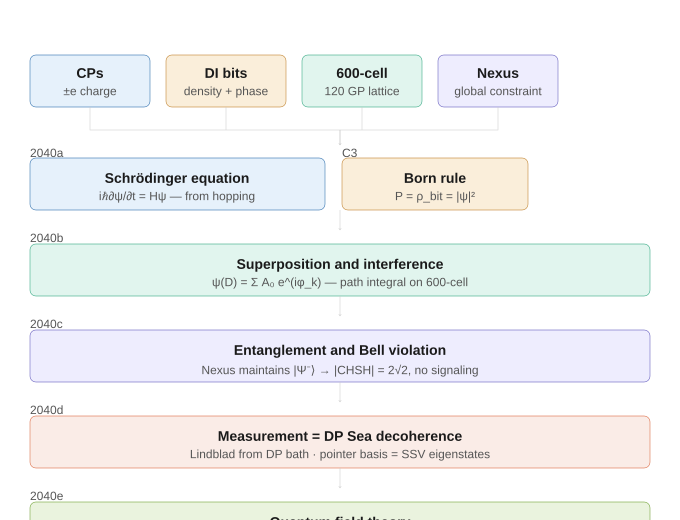
\includegraphics[width=0.90\textwidth]{qm2040f_fig1_emergence_hierarchy.pdf}
\caption{CPP emergence hierarchy.
  The four primitives (top row) funnel into five sequential emergence
  levels (coloured bars), each labelled with the corresponding QM
  series paper number.  Every level inherits from all levels above it.
  The Nexus (purple) plays a distinct role at each level, as
  summarised in Table~1.}
\label{fig:hierarchy}
\end{figure}

%=====================================================================
\ibliographystyle{plainnat}
\ibliography{cpp_qm_series}


\section*{Acknowledgements}
The CPP programme is registered at OSF (DOI:~\url{https://doi.org/10.17605/OSF.IO/JXE8D}) and maintained at GitHub (\url{https://github.com/Hyperphysics-Institute/CPP}).

\bibliographystyle{plainnat}
\bibliography{cpp_qm_series}

\end{document}
